%%%%%%%%%%%%%%%%%%%%%%%%%%%%%%%%%%%%%%%%%
% Beamer Presentation
% LaTeX Template
% Version 1.0 (10/11/12)
%
% This template has been downloaded from:
% http://www.LaTeXTemplates.com
%
% License:
% CC BY-NC-SA 3.0 (http://creativecommons.org/licenses/by-nc-sa/3.0/)
%
%%%%%%%%%%%%%%%%%%%%%%%%%%%%%%%%%%%%%%%%%

%----------------------------------------------------------------------------------------
%	PACKAGES AND THEMES
%----------------------------------------------------------------------------------------

\documentclass[9pt]{beamer}
%\documentclass[9pt]{beamer}

\mode<presentation> {

% The Beamer class comes with a number of default slide themes
% which change the colors and layouts of slides. Below this is a list
% of all the themes, uncomment each in turn to see what they look like.

%\usetheme{default}
%\usetheme{AnnArbor}
%\usetheme{Antibes}
%\usetheme{Bergen}
%\usetheme{Berkeley}
%\usetheme{Berlin}
%\usetheme{Boadilla}
%\usetheme{CambridgeUS}
%\usetheme{Copenhagen}
%\usetheme{Darmstadt}
%\usetheme{Dresden}
\usetheme{Frankfurt}
%\usetheme{Goettingen}
%\usetheme{Hannover}
%\usetheme{Ilmenau}
%\usetheme{JuanLesPins}
%\usetheme{Luebeck}
%\usetheme{Madrid}
%\usetheme{Malmoe}
%\usetheme{Marburg}
%\usetheme{Montpellier}
%\usetheme{PaloAlto}
%\usetheme{Pittsburgh}
%\usetheme{Rochester}
%\usetheme{Singapore}
%\usetheme{Szeged}
%\usetheme{Warsaw}

% As well as themes, the Beamer class has a number of color themes
% for any slide theme. Uncomment each of these in turn to see how it
% changes the colors of your current slide theme.

%\usecolortheme{albatross}
%\usecolortheme{beaver}
%\usecolortheme{beetle}
%\usecolortheme{crane}
%\usecolortheme{dolphin}
%\usecolortheme{dove}
%\usecolortheme{fly}
%\usecolortheme{lily}
%\usecolortheme{orchid}
%\usecolortheme{rose}
%\usecolortheme{seagull}
%\usecolortheme{seahorse}
%\usecolortheme{whale}
%\usecolortheme{wolverine}

%\setbeamertemplate{footline} % To remove the footer line in all slides uncomment this line
\setbeamertemplate{footline}[page number] % To replace the footer line in all slides with a simple slide count uncomment this line
%\setbeamersize{text margin left=7mm,text margin right=7mm} 
\setbeamertemplate{navigation symbols}{} % To remove the navigation symbols from the bottom of all slides uncomment this line
\setbeamertemplate{bibliography item}{\insertbiblabel}
}

\usepackage{graphicx} % Allows including images
\usepackage{booktabs} % Allows the use of \toprule, \midrule and \bottomrule in tables
\usepackage{movie15}
\usepackage{animate}
\usepackage{verbatim}
\usepackage{ amssymb }
\usepackage[english]{babel}
\usepackage{amsthm}
\usepackage{graphicx}
\usepackage{caption}
\usepackage{subcaption}
\usepackage{cancel}
\usepackage{mathdots}
\usepackage{mathrsfs}
\usepackage{relsize}
%\usepackage{enumitem}
\usepackage{float}
\usepackage{cancel}
\usepackage{algorithm}
\usepackage{algorithmic}
\usepackage{color, colortbl}
\usepackage{bm} % For bold greek letters
\usepackage{helvet}
% For bibliography
\usepackage[style = verbose,backend=bibtex]{biblatex}
 \addbibresource{references.bib}
\renewcommand*{\bibfont}{\scriptsize}
% For Matern class figure
\usepackage{tikz,pgfpages,pgflibraryplotmarks}
\usepackage{pgf,pgfplots,pgfarrows} 


\newcommand{\beq}{\begin{equation}}
\newcommand{\eeq}{\end{equation}}
\newcommand{\bseq}{\begin{subequations}}
\newcommand{\eseq}{\end{subequations}}
\newcommand{\beqa}{\begin{eqnarray}}
\newcommand{\eeqa}{\end{eqnarray}}
\newcommand{\calE}{{\cal E}}
\newcommand{\calB}{{\cal B}}
\newcommand{\calC}{{\cal C}}
\newcommand{\calM}{{\cal M}}
\newcommand{\calN}{{\cal N}}
\newcommand{\calF}{{\cal F}}
\newcommand{\hatx}{\hat{x}}
\newcommand{\haty}{\hat{y}}
\newcommand{\tilx}{\tilde{x}}
\newcommand{\tilB}{\tilde{B}}
\newcommand{\tilA}{\tilde{A}}
\newcommand{\bd}{\partial\Omega}
\newcommand{\intO}{\int_{\Omega}}
\newcommand{\intBD}{\int_{\partial\Omega}}
\newcommand{\obs}{u^{obs}}
\newcommand{\tilp}{\tilde{p}}
\newcommand{\tilu}{\tilde{u}}
\newcommand{\tilm}{\tilde{m}}
\newcommand{\hatp}{\hat{p}}
\newcommand{\hatu}{\hat{u}}
\newcommand{\hatm}{\hat{m}}
\newcommand{\arghh}{\!\!\!\! \!\!\!\! \!\!\!\! \!\!\!\!\!\!\!\!}
\newtheorem{proposition}[theorem]{Proposition}
\newcommand*{\QEDB}{\hfill\ensuremath{\square}}


\def\eps{{\varepsilon}}
\def\ie{{\em i.\ e.\ \/}}
\def\cale{{\cal E}}
\def\real{{\bf R}}
\def\rnn{{\real}^{N \times N}}
\def\rmn{{\real}^{M \times N}}
%\def\rnn{{\bf R}^{N \times N}}
%\def\rmn{{\bf R}^{M \times N}}
\def\diag{{\mbox{diag}}}
\def\vf{{\bf f}}
\def\vx{{\bf x}}
\def\vc{{\bf c}}
\def\vd{{\bf d}}
\def\vp{{\bf p}}
\def\vb{{\bf b}}
\def\vy{{\bf y}}
\def\vz{{\bf z}}
\def\ve{{\bf e}}
\def\vs{{\bf s}}
\def\vm{{\bf m}}
\def\vg{{\bf g}}
\def\me{{\bf E}}
\def\mg{{\bf G}}
\def\vw{{\bf w}}
\def\mr{{\bf R}}
\def\mh{{\bf H}}
\def\mc{{\bf C}}
\def\mt{{\bf T}}
\def\ms{{\bf S}}
\def\mi{{\bf I}}
\def\vb{{\bf b}}
\def\vq{{\bf q}}
\def\va{{\bf a}}
\def\vv{{\bf v}}
\def\vu{{\bf u}}
\def\ma{{\bf A}}
\def\mb{{\bf B}}
\def\md{{\bf D}}
\def\vr{{\bf r}}
\def\mm{{\bf M}}
\def\ml{{\bf L}}
\def\mU{{\bf U}}
\def\mv{{\bf V}}
\def\mP{{\bf P}}
\def\mq{{\bf Q}}
\def\mx{{\bf X}}
\def\mf{{\bf F}}
\def\mw{{\bf W}}
\def\mz{{\bf Z}}
\def\bmu{{\bm{\mu}}}
\def\bmgp{{\bm{\Gamma}_{\text{post}}}}
\def\bmgn{{\bm{\Gamma}}}
\def \vsp{{\vs_{\text{post}}}}
\def \vhatm{{\bf \hat{m}}}
\def \vhatu{{\bf \hat{u}}}
\def \vhatp{{\bf \hat{p}}}
\newcommand\p[2]{\frac{\partial #1}{\partial #2}}

\definecolor{Yellow}{rgb}{1,1,0.4}

\setbeamerfont{caption}{size=\scriptsize}


%----------------------------------------------------------------------------------------
%	TITLE PAGE
%----------------------------------------------------------------------------------------

\title[PAT]{Uncertainty Quantification in Photoacoustic Tomography} % The short title appears at the bottom of every slide, the full title is only on the title page

\author{Katrina Petroske, North Carolina State University \\ Jenni Tick, University of Eastern Finlanad \\ Sheroze Sheriffdeen, University of Texas at Austin} % Your name
\institute[G2S3 2108] % Your institution as it will appear on the bottom of every slide, may be shorthand to save space

\date{June 29, 2018} % Date, can be changed to a custom date

\AtBeginSection[]
{
 \begin{frame}<beamer>
 \frametitle{Outline}
 \tableofcontents[currentsection,
    sectionstyle=show/show,
    subsectionstyle=show/show/hide,
    subsubsectionstyle=hide,]
 \structure{\insertsubsection}
 \end{frame}
}

\begin{document}

%%% Slide 1
\begin{frame}
\titlepage % Print the title page as the first slide
\end{frame}

%\begin{frame}
%\frametitle{Overview} % Table of contents slide, comment this block out to remove it
%\tableofcontents % Throughout your presentation, if you choose to use \section{} and \subsection{} commands, these will automatically be printed on this slide as an overview of your presentation
%\end{frame}

%----------------------------------------------------------------------------------------
%	PRESENTATION SLIDES
%----------------------------------------------------------------------------------------


%%% Slide 2
\section{Background}
%Outline Slide

%----------------------------------------------------------------------------------------
%%% Slide 3
\subsection{PAT}
\begin{frame}
\frametitle{Photoacoustic Tomography  (PAT)}
\begin{columns}
	 \begin{column}{.5\textwidth}
	 	\begin{figure}
 			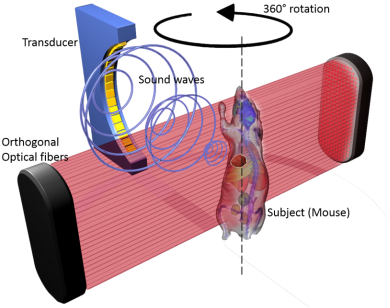
\includegraphics[width = \linewidth]{mouseSetup.png}
 			\caption{Setup of PAT \footnotemark.}
		\end{figure}
 	\end{column}
  	\begin{column}{.5\textwidth}
		\begin{figure}
 			\animategraphics[autoplay,loop,width=0.65\linewidth]{10}{rot_mouse}{}{}
 			\caption{Image of a mouse's vascular system produced with PAT$^1$ . }
		\end{figure}
	\end{column}
\end{columns}
\vspace{-2mm}
\hspace{-4mm}\textbf{Why PAT?}
\begin{columns}
	 \begin{column}{.6\textwidth}
                \begin{itemize}
                \item can be used for breast and brain imaging
                \item low monetary cost
                \end{itemize}
 	\end{column}
  	\begin{column}{.5\textwidth}
	      \begin{itemize}
                \item safe for variety of patients
                \item can do functional imaging
                \end{itemize}
	\end{column}
\end{columns}

\footcitetext{tomo}

\end{frame}

%%% Slide 4
%----------------------------------------------------------------------------------------
\subsection{Model}
%\begin{frame}
%\frametitle{Diffusion Equation}
%
%\begin{columns}
%	 \begin{column}{.35\textwidth}
%	 \textbf{Diffusion Equation:}
%            \begin{align*}
%            -\nabla \cdot (\gamma \nabla u) +\sigma u  &= 0 \;\;\;\text{ in } \Omega\\
%            u  &= g\;\;\; \text{ on } \bd
%            \end{align*}
% 	\end{column}
%  	\begin{column}{.5\textwidth}
%		\begin{figure}
%			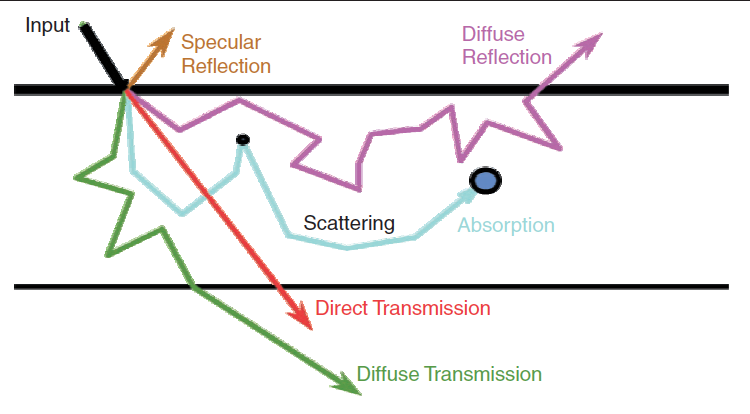
\includegraphics[width = \linewidth]{light.png}
%			\caption{Possible ways a photon can interact with medium\footnotemark.}
%		\end{figure}
%%	\begin{figure}
%% 		\includegraphics[width = \linewidth]{absorp.png}
%% 		\caption{Absorption spectrum of oxygenated and deoxygenated hemogloblin. \cite{DOT}}
%%	\end{figure}
%	\end{column}
%\end{columns}
%Note: This is an approximation of the radiative transport equation
%
%\begin{columns}
%	 \begin{column}{.5\textwidth}
%\begin{itemize}
%\item $u$ is the photon density 
%\item $g$ is the source 
%\end{itemize}
% 	\end{column}
%  	\begin{column}{.5\textwidth}
%\begin{itemize}
%\item  $\sigma$ is the absorption coefficient
%\item $\gamma$ is the diffusion coefficient 
%\end{itemize}
%	\end{column}
%\end{columns}
%\footcitetext{DOT}
%\end{frame}
%
%-------------------------------------------------------------------------------------
%%% Slide 5
\subsection{}
\begin{frame}{Wave Equation}

\textbf{Wave Equation:}
\begin{align*}
\frac{1}{c^2} p_{tt} - \Delta p &= 0,\;\;\;\;\;\;\;\text{ in } \Omega \times (0, T] \\
p(0,x) & = H(x),\;\text{ in } \Omega  \\
p_t(0,x) &= 0, \;\;\;\;\;\;\;\text{ in } \Omega 
\end{align*}
and 
\[
H(x) = \Upsilon(x) \psi(x)
\]
where 
\begin{itemize}
\item $p$ is the pressure
\item $c$ is the wave speed
\item $H$ is the initial pressure
\item $\Upsilon$ is the Gr\"{u}neisen parameter (measure of efficiency)
\item $\psi$ is the absorbed energy
\end{itemize}

\end{frame}


%-------------------------------------------------------------------------------------
%%% Slide 6
\subsection{}
\begin{frame}
\frametitle{Coupled}
\begin{columns}
	 \begin{column}{.5\textwidth}
    	 \textbf{Diffusion Equation:}
                \begin{align*}
                  -\nabla \cdot (\gamma \nabla {\color{red} u}) +{\color{blue} \sigma} {\color{red} u}  &= 0 \;\;\;\text{ in } \Omega\\
            	{\color{red} u}  &= g\;\;\; \text{ on } \bd
                \end{align*}
                \begin{itemize}
            	\item ${\color{blue} \sigma}$ is the absorption coefficient
            	\item $\gamma$ is the diffusion coefficient 
            	\item $\color{red} u$ is the photon density 
                 \end{itemize}
 	\end{column}
  	\begin{column}{.5\textwidth}
            \textbf{Wave Equation:}
            \begin{align*}
            \frac{1}{c^2} p_{tt} - \Delta p &= 0\;\;\;\text{ in } \Omega \times (0,T] \\
            p(0,x) & =  \Upsilon {\color{blue} \mu} {\color{red} u} \;\;\;\text{ in } \Omega \\
            p_t(0,x) &= 0 \;\;\;\text{ in }  \Omega
            \end{align*}
            \begin{itemize}
            \item $\Upsilon$ is the Gr\"{u}neisen parameter (measure of efficiency)
            \end{itemize}
	\end{column}
\end{columns}
\vspace{5mm}
They are coupled by the initial pressure
\[
H(x)  = \Upsilon(x) \psi(x) = \Upsilon(x) {\color{blue}\mu} (x) {\color{red} u} (x)
\]
\\~\\
\pause
Goal: Find the posterior distribution of the initial pressure
\end{frame}

%-------------------------------------------------------------------------------------
%%% Slide 7
\section{Method}
%----------------------------------------------------------------------------------------


%%% Slide 8
\subsection{}
\begin{frame}
\frametitle{Preliminaries}
\begin{itemize}
\item Discretize w.r.t time and find the weak form 
\item Solve the forward problem in FEniCS
\end{itemize}
\begin{figure}
	\centering
	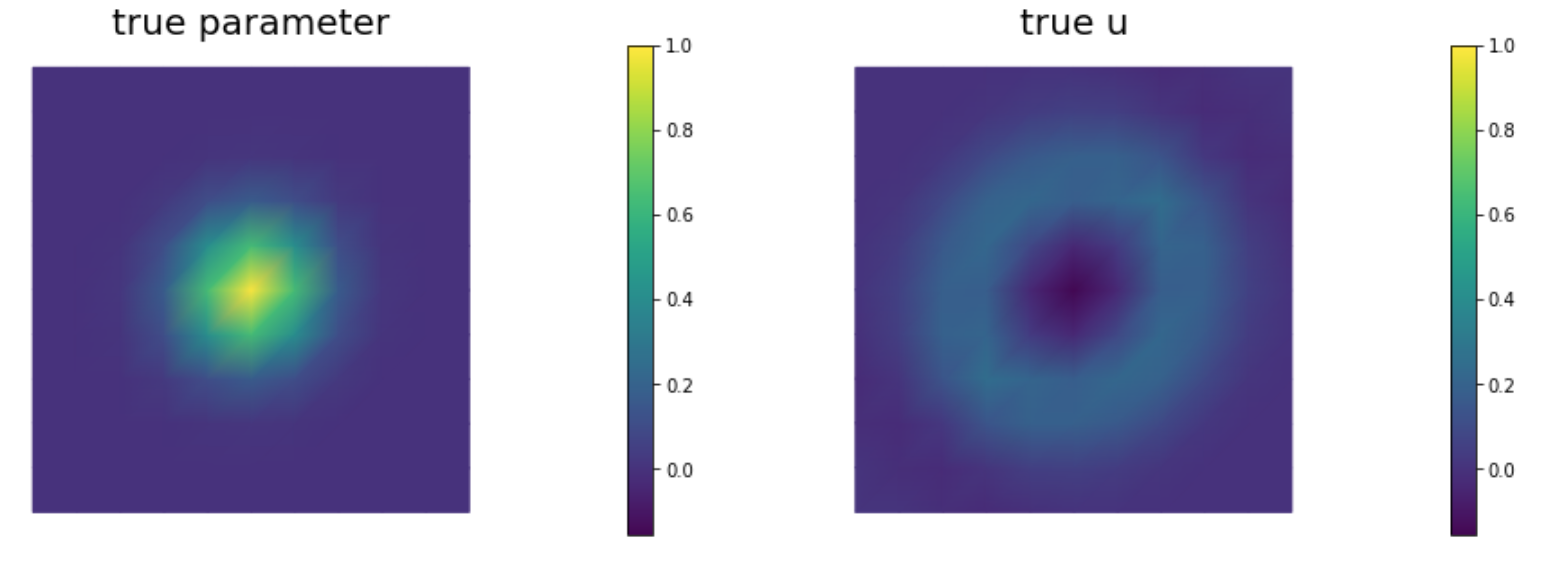
\includegraphics[width = \linewidth]{true.png}
	\caption{True initial pressure and true solution.}
\end{figure}
Grid size is 121 $\implies$ 121 parameters
\end{frame}
%----------------------------------------------------------------------------------------
%%% Slide 
\subsection{}
\begin{frame}
\frametitle{Method - MCMC}
Using MUQ 
\begin{itemize}
\item Prior with Matern kernel (v=1/2) with a linear mean 
\item Gaussian likelihood
\end{itemize}
\vspace{3mm}
 We tried 
 \begin{itemize}
 \item Adaptive Metropolis Algorithm
 \item Preconditioned Crank Nicolson
 \item Random Walk Metropolis 
 \end{itemize}

\end{frame}

%----------------------------------------------------------------------------------------
%%% Slide 
\subsection{Whole field measurements}
\begin{frame}
\frametitle{Method - MCMC}
 Assuming whole field measurements at the final time
\begin{figure}
\hspace{-1cm}
\begin{subfigure}{0.3\textwidth}
\vspace{-0.3cm}
	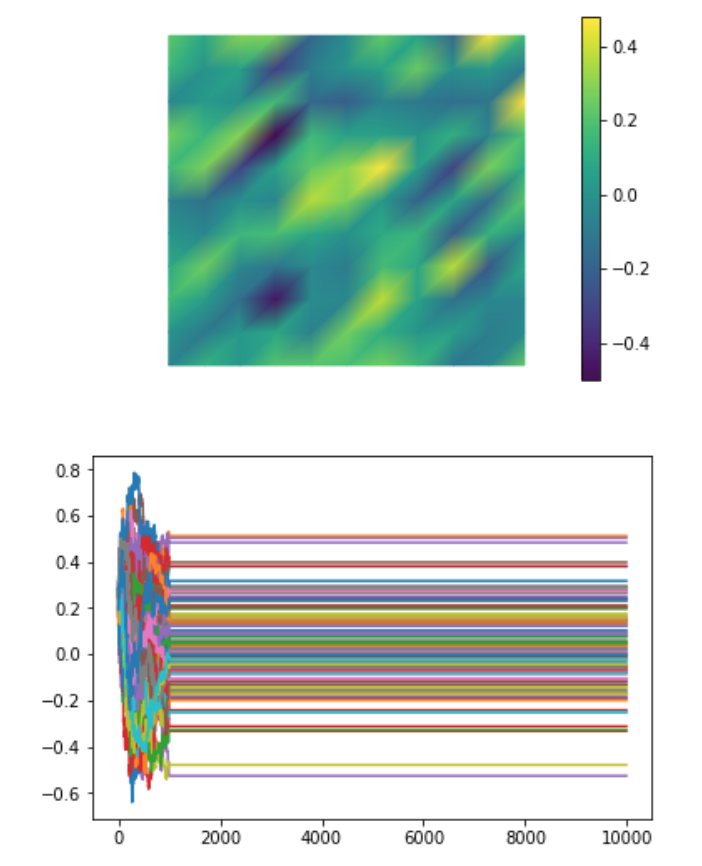
\includegraphics[scale = 0.3]{AM_noObs.png}
	\caption{Adaptive Metropolis.}
\end {subfigure}
\hspace{0.7cm}
\begin{subfigure}{0.3\textwidth}
	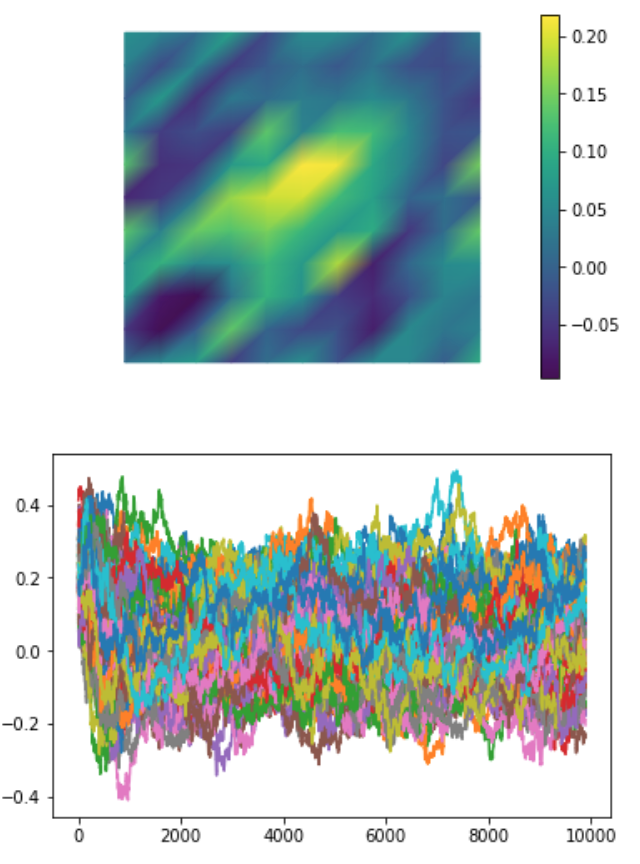
\includegraphics[scale = 0.3]{MH_noObs.png}
	\caption{Preconditioned Crank Nicolson.}
\end{subfigure}
\hspace{0.6cm}
\begin{subfigure}{0.3\textwidth}
	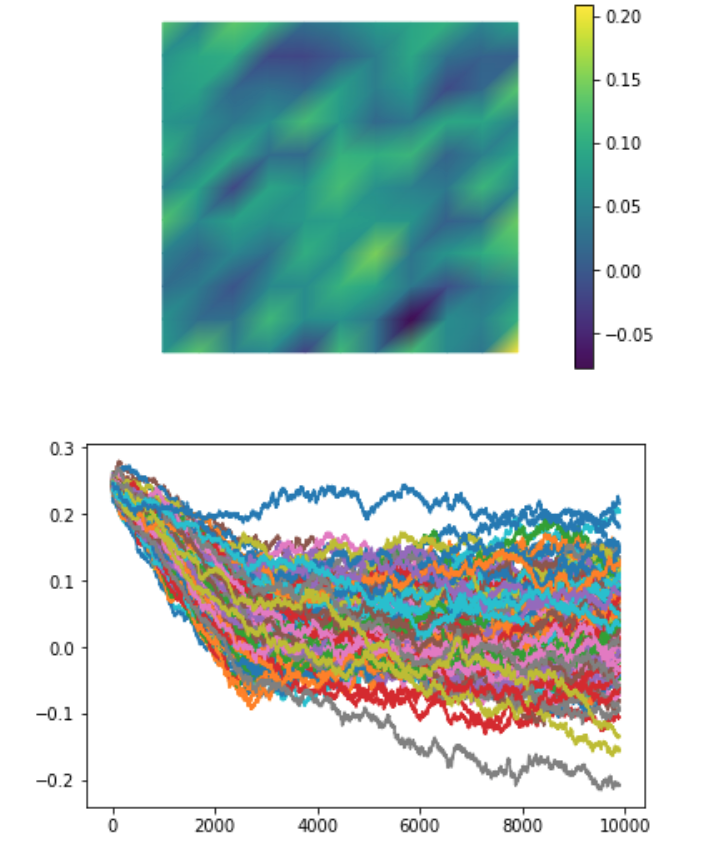
\includegraphics[scale = 0.3]{pCN_noObs.png}
	\caption{Random Walk Metropolis.}
\end{subfigure}
\end{figure}

\end{frame}


%----------------------------------------------------------------------------------------
%%% Slide 
\subsection{Discrete Sensors}
\begin{frame}
\frametitle{Method - MCMC}
Sensors taking measurements at multiple times

\begin{figure}
\hspace{-2cm}
\begin{subfigure}{0.3\textwidth}
	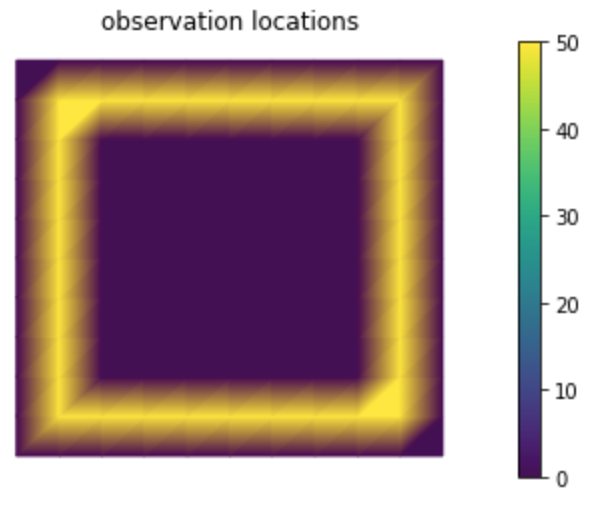
\includegraphics[scale= 0.45]{obs_loc.png}
\end{subfigure}
\hspace{2.5cm}
\begin{subfigure}{0.25\textwidth}
	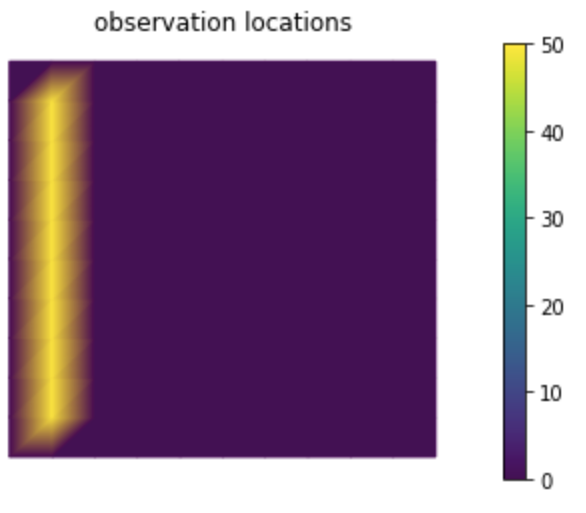
\includegraphics[scale= 0.45]{obs_loc_1side.png}
\end{subfigure}
\end{figure}


\end{frame}


%----------------------------------------------------------------------------------------
%%% Slide 
\subsection{}
\begin{frame}
\frametitle{Method - MCMC}
Observing at multiple times at sensor locations
\begin{figure}
\hspace{-1cm}
\begin{subfigure}{0.3\textwidth}
\vspace{-0.3cm}
	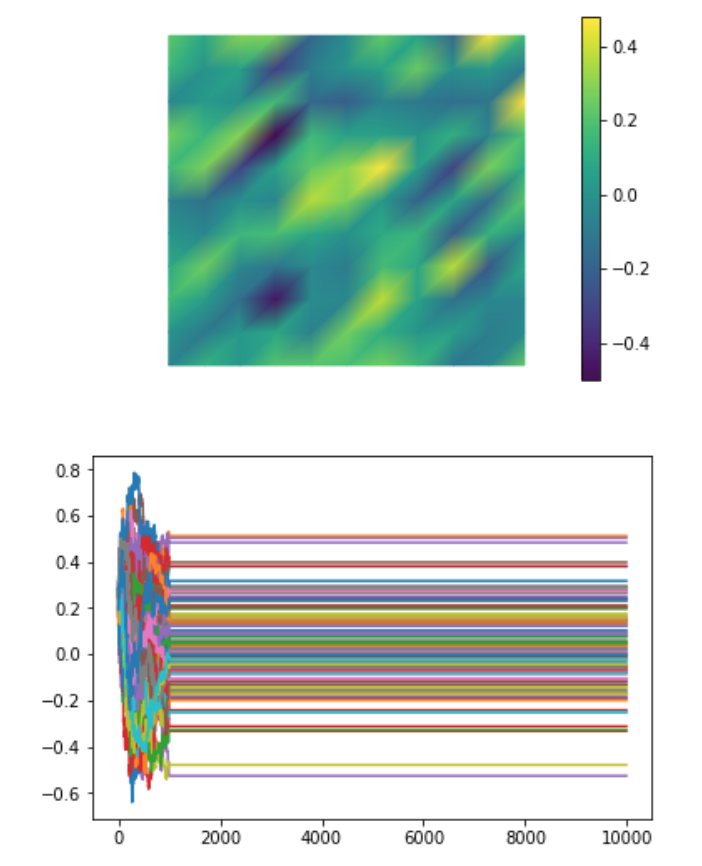
\includegraphics[scale = 0.3]{AM_noObs.png}
	\caption{Adaptive Metropolis.}
\end {subfigure}
\hspace{0.7cm}
\begin{subfigure}{0.3\textwidth}
	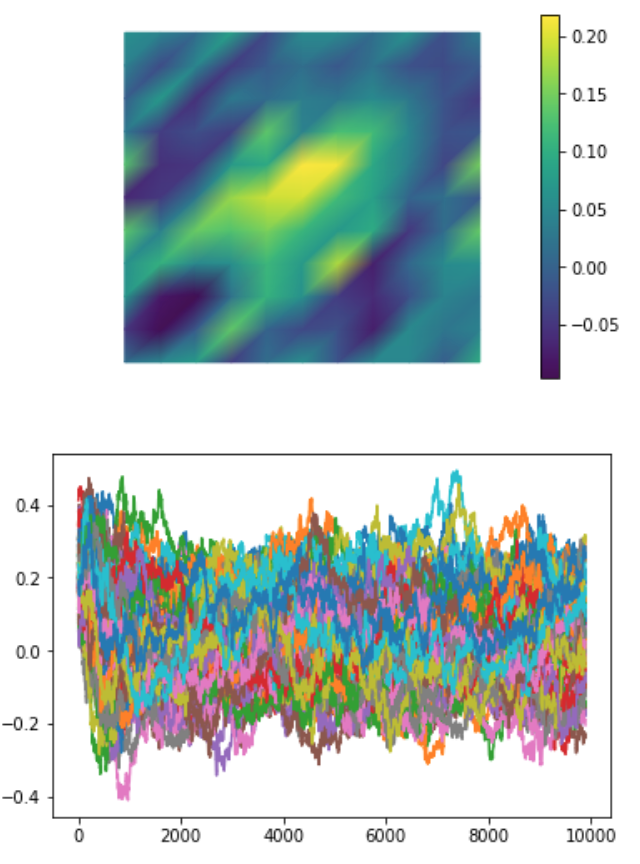
\includegraphics[scale = 0.3]{MH_noObs.png}
	\caption{Preconditioned Crank Nicolson.}
\end{subfigure}
\hspace{0.6cm}
\begin{subfigure}{0.3\textwidth}
	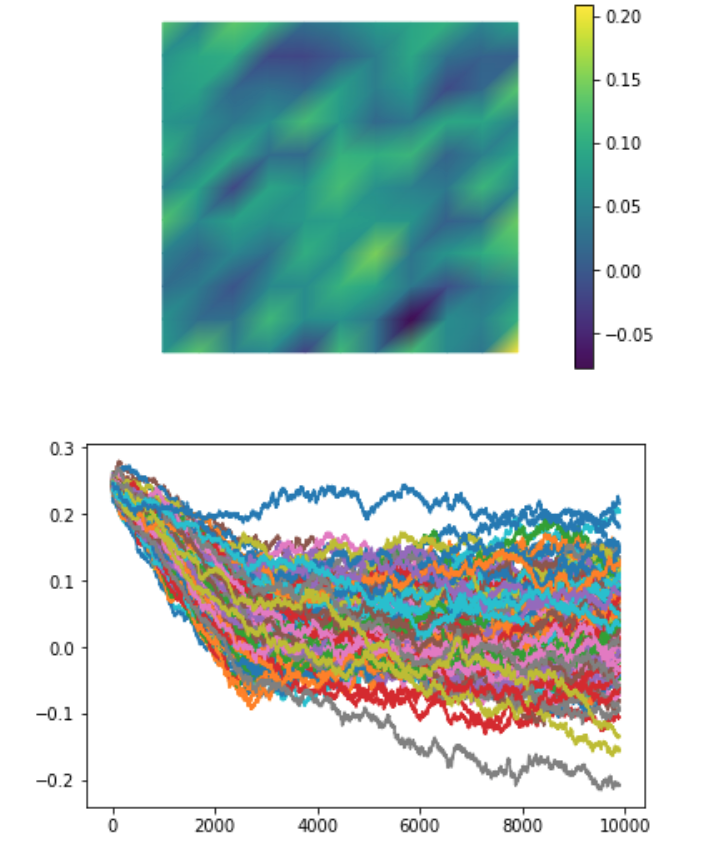
\includegraphics[scale = 0.3]{pCN_noObs.png}
	\caption{Random Walk Metropolis.}
\end{subfigure}
\end{figure}

\end{frame}


%----------------------------------------------------------------------------------------
%%% Slide 
%\section{Acknowledgements and References}
\subsection{}
\begin{frame}[allowframebreaks]
\frametitle{Acknowledgements and References}
\underline{Acknowledgements:} \\~\\
Thanks to Matt, Georg, Youssef, Umberto, and Omar
\\~\\

\nocite{fenics2} 
\nocite{hippylib}
\nocite{numopt}
\underline{References:} \\~\\
%\bibliographystyle{siam}
\small{
\printbibliography
}
\end{frame}


%------------------------------------------------

\begin{frame}
\vspace{3cm}
\Huge{\centerline{Questions?}}
\vspace{3cm}
\end{frame}

%----------------------------------------------------------------------------------------



\end{document} 



